\chapter{Main Work}
\label{chp:quickrollout} 

Make a best practice for quick roll out, by the use of a MultiBox. 

\section{Set-up of the Mesh Potatoes}
%Flashing process
%How did we get Internet to the network?
%Hvordan en MP kan koble seg til de ulike uplinkene?
%3G via TP-links til mesh nettverket?

\section{The Emergency Box}

\begin{center}
\begin{table}[!ht]
\caption{\label{tab:components}The components of MultiBox}
    \begin{tabular}{ | l | p{9cm} |}
    \hline
    \textbf{Component} & \textbf{Description and purpose} \\ 
    \hline
    Mesh Potato &  \\ 
    \hline
    Suitcase/box &   \\ 
    \hline
    Power supply & \\
    \hline
    Plain old telephone & \\
	\hline
	Junction box & \\
	\hline
	Solar panel & \\
	\hline
	Solar panel regulator & \\
	\hline
    \end{tabular}
   \end{table}
\end{center}

%How is the box set up?
%How is it made?
%How does it work?
%Explain the different components
%Explain evt. changes
%Script?

\section{Up-Link}
Our main focus when deploying the emergency boxes, is to provide Internet to the mesh network. This is because it is crucial to have the possibility to communicate with the local community and the outside world during an emergency situation. In 2011, UN declared Internet access a Human Right \cite{HR}. This says something about the extent of the Internet, and the importance of connectivity. In order to provide Internet to the mesh network formed by the emergency boxes, at least on the the Mesh Potatoes must be connected to an access network via an uplink. An uplink connects a device or a LAN to a larger network \cite{uplink}. Which type of access network that is available depends of the location. Some places there might exist a stable landline, other places not. Then an option could be to use satellite or cellular networks. It is therefore important that the emergency box has high adaptability in order to fit different scenarios. The availability of the different uplinks is not the only thing that vary. The up-link speed and the price also varies from place to place, but also varies between the types of uplinks. In the following sections, we will look at some of the uplinks available, and how Internet access can be provided to the mesh network.  

%I hvilke tilfeller de passer best? 
%Hva slags utstyr for hver up-link må til??

\subsection{Internet via Telephone-line}
The most common way of getting Internet access is via a landline. The telephone lines are most often used for this, since they can be converted to broadband. In this way it can be used for phone calls and Internet simultaneously \cite{internet}. The line is usually in the form of twisted pairs (copper lines). These lines support broadband up to 10 Mbps, and are often in form of ADSL, or other digital subscriber line of type x (xDSL) technologies \citep{audestad}. Internet via telephone lines can be provided as a stand-alone solution, or it can be provided together with television or/and phone service. The latter option is usually cheaper. Internet through landlines have a high reliability \cite{cablevssatellite}. We will now shorty describe some technologies for getting Internet access via a telephone line; dial-up Internet connection, ISDN, and DSL. Although dial-up Internet connection is practically extinct in many countries, we will include it here due to the different application scenarios for the emergency box. 

\paragraph{Dial-up Internet connection}
Dial-up is an analogue technology that utilizes the telephone line. A telephone wall jack is used as a fixed point of connection, and the computer is connected to a voiceband modem. With this technology, the data is transmitted over the same frequencies used for phone calls. Hence, if you only have one telephone line, you cannot take a phone call and use Internet at the same time \cite{differentuplinks}. Along with the digital era, better internet technologies were introduced; ISDN and DSL. 

\paragraph{ISDN}
Integrated Services Digital Network (ISDN) is a fixed internet connection, which also utilizes the telephone lines. When using ISDN, as with dial-up, a telephone wall jack is used as a fixed point of connection. But ISDN utilizes a ISDN terminal adapter instead of voiceband modem. This ISDN terminal adapter sends out digital signals. The data speed varies between 64 Kbps - 129 Kbps. The speed of the data is symmetric, which means upstream and downstream data rates are the same. In contrary to dial-up, ISDN allows voice calls and transmission of data simultaneously. ISDN is faster than dial-up, but the speed is nothing compared to the speed obtained using DSL \cite{differentuplinks}. 

\paragraph{DSL}
Digital subscriber line (DSL) is, like the name insinuates, a digital high-speed technology for Internet access that allows simultaneous voice and data transfer. Like dial-up and ISDN, DSL also run over the telephone lines. With DSL the data is not converted between analogue and digital signals. Despite this, the signals are modulated in order to be transferred on non-voice frequencies. DSL is an always-on technology, and differ from the previous technologies mentioned in this way. Only a small part of the telephone line is used for voice signals. The DSL technology allows utilization of a unused frequency spectrum of an telephone line, hence making it possible to transmit data faster. When the voice and data signals arrive at the telephone company's local switching station, they are separated and routed differently; voice to regular telephone system and data to the ISP, and then the Internet. A connection must be within approximately 5 kilometres of a station in order for DSL to work. The speed depends on many factors. Data can be transported up to 6 Mbps (distance of approximately 2 kilometres). Relevant factors that have an impact on the speed is distance to the switching station and the quality of the telephone line. Like mentioned earlier, there are different types of DSLs. The most common is ADSL, where the A stands for asymmetric; the downstream speed is faster than the upstream speed \cite{differentuplinks}.

\subsection{Mobile Network Technologies}
It is getting more and more common to use cellular technologies for broadband. Through mobile network technologies, high-speed Internet access can be provided via portable devices. The only thing required to get Internet access from mobile networks is having a GSM or CDMA-based cellular service available. 

Mobile networks provide wireless high-speed Internet access. Wherever there is GSM or CDMA-based cellular services available

%What is mobile broadband?
%Mobile broadband technology, also called wireless wide area network (WWAN) technology, provides wireless high-speed Internet access through portable devices.  With mobile broadband, you can connect to the Internet from any location where there is GSM or CDMA-based cellular service available for mobile Internet connectivity. With mobile connectivity, you can maintain your Internet connection even as you move from place to place.

%Mobile broadband is available with most 2G, 2.5G, and 3G cellular and mobile networks.
%http://windows.microsoft.com/en-us/windows7/what-is-mobile-broadband




%3G offers a "always-on" 
%Cellular networks normally provide broadband connections suitable for mobile access. The technologies in use today fall into two categories - 3G (third generation cell networks) and 4G (fourth generation).
%Types of 3G broadband include: Enhanced Data GSM Environment (EDGE), EV-DO, and High-Speed Downlink Packet Access (HSPA). WiMax and LTE represent 4G broadband.
%Beside phones, Internet and network access using these technologies is increasingly being incorporated into laptop computers, automobiles and public transportation.

%Limitations of Mobile Broadband
%Along with the obvious advantage of Internet access from anywhere, consider these common limitations of mobile broadband: monthly service plans can cost significantly more than for traditional broadband, sometimes including extra fees for larger volumes of data usage "high speed" can mean significantly slower than for traditional broadband, sometimes less than 1 Mbps depending on the service provider's network capability network outages occur when roaming, caused by limits of the service provider coverage area or obstructions from geography, and service may also be disrupted inside larger buildings due to interference
%http://compnetworking.about.com/od/internetaccessbestuses/f/what-is-mobile-broadband.htm

\subsection{Satellite}
%ulovlig i feks india, hva skjer da? http://en.wikipedia.org/wiki/Satellite_phone

Internet from satellites are offered by a satellite Internet provider \cite{cablevssatellite}. The satellite are orbiting the Earth, and get signals from a land based Internet connection. To get Internet access via satellite you need a satellite dish. The main advantage of using satellite is that it provides an universally available Internet access \cite{broadband}. Since it is universally available, it is fitted for use in rural regions where there exists no landlines or other options for connecting to the Internet. But like with everything else, there also exists disadvantages with using satellite-Internet. Since it is a shared medium, privacy concerns arise, and the speed are dependent of simultaneous use. Also the connection can be affected by bad weather, unlike for a wired connection, hence it is not as reliable as cable. 

\subsection{Summary Up-Links}

\begin{center}
\begin{table}[!ht]
\caption{\label{tab:uplinks}Advantages and disadvantages - Up-links \cite{}.}
    \begin{tabular}{ | l | p{4cm} | p{5cm} |}
    \hline
    \textbf{Up-links} & \textbf{Advantages} & \textbf{Disadvantages} \\ 
    \hline
    Landline/xDSL & High reliability, cheap, & Low availability in rural areas \\ 
    \hline
     Cellular networks & High availability & Expensive\\
    \hline
    Satellite & High availability  & Not as reliable as cable, and generally more expensive than cable \\ 
    \hline
    \end{tabular}
   \end{table}
\end{center}

\subsection{Apple's Mesh Network}
In March 2014 a new iOS app was released, FireChat. This app enables the possibility to chat with people "off-the-grid" \cite{fireChat}. FireChat utilizes Apple's Multipeer Connectivity Framework introduced in iOS7 \cite{appleMesh}. The Multipeer Connectivity framework provides support for discovering services provided by nearby iOS devices using peer-to-peer Wi-Fi, infrastructure Wi-Fi networks and bluetooth to communicate with those services. This communication could either be message-based data, streaming data and resources such as files \cite{multipeer}. These technologies have a short range, but this range can be greatly extended by a chain of users that creates a mesh network, see section \ref{subsec:mesh} for more information about mesh networks. AirDrop is a product that have been out there for a little while and also utilizes mesh networks. The Main difference is that FireChat is fully decentralized and peer-to-peer. When there are multiple users in one area FireChat relay messages in the same way as Internet, from node to node, just in this case it is from phone to phone.  This, not only, enables two users to chat with each other without Internet connection, but also far beyond Wi-Fi and Bluetooth range from each other, using the chain of users (phones). For example if Bob is connected to Alice, and Alice is connected to Carol, Bob and Carol can send messages to each other. This chain can be indefinitely long. As long as no one device goes out of Wi-Fi range, all the devices can communicate with each other. 

This new framework will mainstream wireless mesh networking. Internet can now become available in places where it earlier was non existent. This could for example be a hotel basement, cave or rural areas where there are no cellphone towers, or disaster situations where Wi-Fi or mobile broadband  is no longer available. There are many benefits with the use of mesh networks. Mesh networks does not require a centralized infrastructure, there are no need for all the devices to be connected to a access point (as a router). Another benefit is that the mesh network is really easy to set up - everybody just uses the app FireChat (or similar applications like AirDrop), the network is created and everybody is connected. Simple as that! 

The possibilities for this feature are enormous. Both in the creation of applications but also the area of usage. In a lot of countries Internet and mobile broadband connection is extremely expensive, people might afford a used cellphone but not the cost to connect. With this new feature Internet connectivity can be spread through the mesh network needing only one node (phone) to have internet access. This way of spreading connectivity can open the possibility for people in rural, poorer areas like slums and small villages to stay connected. But not only the poor and rural areas can benefit from this new mesh-networking feature. Young people that does not have a phone can use an iPad or similar to talk to their friends. Or teens with restricted cell contracts can still connect with their friends, just with the help of the neighbours kids phone. Since FireChat enables communication without the use of internet it can be a useful tool to communicate privately and also to send sensitive data.
 
It is not only Apple that is seeing the enormous potential in main-streaming mesh networking. Google has also expressed that they are working on a home mesh network \cite{googleMesh}. FireChat and AirDrop is just the beginning. We believe more extensive and mind blowing applications are to come. 


\subsection{Internet Balloons}
The majority of the world today is not connected to the internet. Two thirds of the worlds population does not have access to the Internet. Project Loon, a Google project, is a network of high altitude balloons travelling in the stratosphere, and through this network be able to give Internet to the Entire world. Cost effective, reliable and inexpensive internet connection to everybody. The project started in June 2013 as a experiment in New Zealand \cite{loon}. 

\begin{figure}
        \centering
        \begin{subfigure}[t]{0.43\textwidth}
                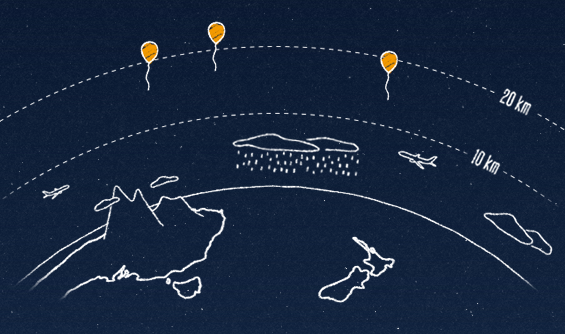
\includegraphics[width=\textwidth]{loon2.PNG}
                \caption[The Balloons are situated in the stratosphere]{\textbf{The Balloons are situated in the stratosphere.}} 
                \label{fig:loonStratosphere}
        \end{subfigure}%
        ~ %add desired spacing between images, e. g. ~, \quad, \qquad etc.
          %(or a blank line to force the subfigure onto a new line)
        \begin{subfigure}[t]{0.415\textwidth}
                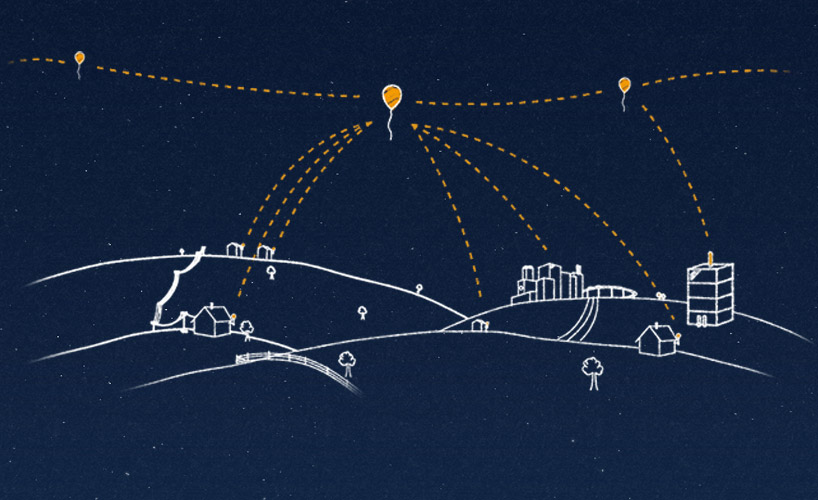
\includegraphics[width=\textwidth]{loon1.jpg}
               \caption[Connecting to the Internet]							{\textbf{Connecting to the Internet}} 
                \label{fig:loonConnect}
        \end{subfigure}
        ~ %add desired spacing between images, e. g. ~, \quad, \qquad etc.
          %(or a blank line to force the subfigure onto a new line)
        \caption{Project Loon: Balloon-powered internet for everyone.}\label{fig:loon}
\end{figure}

The balloons are 15 meter in diameter. They travel about 20 km up in the air, in the stratosphere, twice as high as airplanes and weather, this is shown in \fref{fig:loonStratosphere}. At this altitude there are many layers of wind, each varies in direction and speed. By regulating which wind the balloons are flying in it is possible to control their position, and steer them in the desired direction. \fref{fig:loonConnect} show that  people can connect to the Internet shared by the balloons by having a special antenna attached to their house. From this antenna the signal bounces to one balloon which again bounces through the other balloons and down to the Local Internet Provider on earth. This creates a network in the sky. 

In order to control the altitude of the balloon, there is a special designed control system is designed. The system is controlled remotely from the ground. By either pumping air in or letting air out the balloon, one can decide in what layer of air the balloon should be in. Letting air in and out is not the only way to decide is the balloon should go up or down, but it is the only way to do so in huge scale. A GPS is attached each balloon in order to keep track of precise positions and see how the winds are changing. There are enormous amounts of data collected. The balloons are flying at the same speed as the wind.  

The balloons contains specially designed antennas and radio. This in order to receive signals from Project Loon only, in order to achieve high bandwidth over land distances. 
Satellites are geostationary and stay at the same place and at the same altitude.This means that the satellite dish can be mounted in the right direction. This is not the case with the balloons, they move and they also vary in attitude. A fixed pointing dish would therefore not work. The antenna needs more sensitivity to an angle than it does straight up, which results a uniform signal strength. 

Since the balloons are in constant movement, it is important to make sure that there allays is a balloon available and one ready to move in when one move out so that the connectivity always are available. If not this project would not be of much use. Every balloon contains information about all the other balloons in order to spread out nicely. Think of it as a flock of birds, they always look at the one next to them and space out nicely.

The balloons are solely run on solar power and are controlled by a mission control on earth. The balloon works as a communication tower in the sky. The solar panels catches the sunlight that is available running the day, as well as charging up the lithium-ion battery to last the night. In the stratosphere it is -70 degrees Celsius, these extreme cold conditions are not ideal fro the lithium battery. In order to make sure that the battery does not loose its effective battery capacity it is important that the battery is kept warm. The battery pack is insulated to reflect the heat that comes of the electronics to stay warm. This is still under development. 

When it comes to lifetime, the goal is that the balloons stay alive for a 100 days, or 3 laps around the globe. It is important to make sure that the balloon is leak free. The material is under a lot of stress, air is constantly being pumped in and out to control the position of the balloons. As well as the extreme cold and warm temperatures. 

Bot on the way up and down the air traffic control in the specific country have to be contacted since they go through airspace. Project loon requested permission to land on Norwegian soil according to Teknisk Ukeblad, a Norwegian science magazine. This permission was approved. \cite{loonTU}

\section{Different Scenarios Where a Quick Roll-out is Necessary}
%What are the specific need for the different scenarios? What adjustments are necessary?

Everyday there are situations all over the world that in some way affects the modern communications systems, or causes a need for one. These situations can range in everything from big natural disasters like the tsunami in Japan or the volcano outbreak in the Philippines, where either parts of the communication system is not functioning or there is a desperate need for one. To temporary refugee camps and IDP camps, and situations where a mobile tower is down, or blackouts. Also more festive situations can have use of the quick roll-out system. Imagine a big group gathered at a festival in another country. It is expensive to call or use mobile data, to be able to use cheap internet via the mesh Potatoes would save the users for a lot of money. 

\subsection{Natural Disasters}
%Asia og Sør-Amerika
%Philippines - contact Kenneth Bjerkelund to find out their needs for internet etc. makingchange.no. 
A Natural disaster id defines as; \textit{any event or force of nature that has catastrophic consequences, such as avalanche, earthquake, flood, forest fire, hurricane, lightning, tornado, tsunami, and volcanic eruption} \cite{naturalDisaster}.


\subsection{Blackouts}

\subsection{Temporary Refugee and IDP camps}
Not all refugee and IDP camps are as well established, like the ones in Dadaab. Many camps are temporary, and are therefore in more need of a temporary communication system. 

\subsection{Breakdown of Mobile Towers}


The 10th of June 2011 one of Telenor had problems with one of its servers in Oslo. This problem caused a down time of 18 hours and affected 3 000 000 Telenor users \cite{listeNedetid}. Not only was this the biggest problem Telenor have had since they opened their mobile network in 1993, but also the longest downtime and highest number of affected users recorded in Norway. In addition to this it all happened in a period with severe flooding in big parts of the eastern Norway, and made it difficult to reach emergency numbers. The fact that the problems occurred during the flooding just made the situation much worse. \cite{TelenorNede}

\subsection{Mountain Areas - Avalanches}

\subsection{Festivals}

\subsection{Differences/relation between different scenarios}
%What kind of adjustments are needed between the different scenarios?


%Mopedtilfellet
%Raspberry Pi


\section{The Process of Quick Roll-out}

\subsection{How are telephone numbers assigned?}
%How do people know what number to call?

\subsection{Training of People}
